\documentclass{beamer}
\usetheme[titleformat=regular,sectiontitleformat=regular,frametitleformat=regular]{m}

\usepackage[brazil]{babel}
\usepackage[numberedbib]{apacite}
\usepackage[utf8]{inputenc}
\usepackage{mathabx}
%\usepackage{amsmath}
\usepackage{tabularx}
\usepackage{lipsum}
\usepackage{multicol}
\usepackage{media9}

\newcommand\Fontvi{\fontsize{7}{7.2}\selectfont}


\title{A New Metaheuristic Bat-Inspired Algorithm }
\date{\today}
\author{Acadêmico: Herberth Amaral \\
Disciplina: Computação evolutiva \\
Prof. Dr. João Batista Menes}
\institute{Programa de Pós-Graduação em Modelagem Computacional e Sistemas - UNIMONTES}
\begin{document}
  \maketitle

  \begin{frame}{Introdução}
      Algoritmos de metaheurística inspirados em enxames de partículas (pássaros, peixes, abelhas, formigas, etc) ajudam a resolver problemas difíceis.
  \end{frame}

  \begin{frame}{Introdução}
      \includemedia{Vídeo - Exemplo de otimização por enxame de partículas}{pso.mp4}
  \end{frame}

  \begin{frame}{Introdução}
      O artigo desta apresentação apresenta uma nova abordagem baseada na ecolocalização de \textbf{morcegos}, especialmente morcegos pequenos (os maiores não se orientam tanto via ecolocalização).
  \end{frame}

  \begin{frame}{Biologia da metaheurística}
      \begin{itemize}
          \item Localização por sonar, chamado de \textbf{ecolocalização};
          \item Frequencia constante na região de 25kHz até 150kHz;
          \item Cada pulso emitido dura entre 5 e 20ms, 10 a 20 vezes por segundo chegando até 200 por segundo quando próximo de uma presa;
      \end{itemize}
  \end{frame}

  \begin{frame}{Algoritmo}
      \begin{itemize}
          \item Todos os morcegos usam ecolocalização para sentir distância;
          \item Morcegos voam aleatoriamente com velocidade $v_i$ na posição $x_i$ com uma frequencia fixa $f_{min}$, tamanho de onda $\lambda$ e estridência variável $A_0$. Eles podem ajustar o tamanho de onda dos pulsos e ajustar a taxa de emissão $r \in [0,1]$ dependendo da proximidade do alvo;
          \item Apesar da estridência variar de várias formas, assumimos que varia de um valor (positivo) alto $A_0$ até um valor mínimo constante $A_{min}$
      \end{itemize}
  \end{frame}

  \begin{frame}{Modelagem matemática}

      \begin{equation}
          \lambda = \dfrac{v}{f}
      \end{equation}

      \begin{equation}
          f_i= f_{min} + (f_{max} - f_{min})\beta, \beta \in [0,1],
      \end{equation}

      \begin{equation}
          v^{t}_i = v^{t-1}_i + (x^{t}_i - x_*)f_i,
      \end{equation}

      \begin{equation}
          x^{t}_i = x^{t-1}_i + (v^{t}_i)
      \end{equation}

  \end{frame}


  \begin{frame}{Algoritmo}
      \begin{figure}
          \centering
          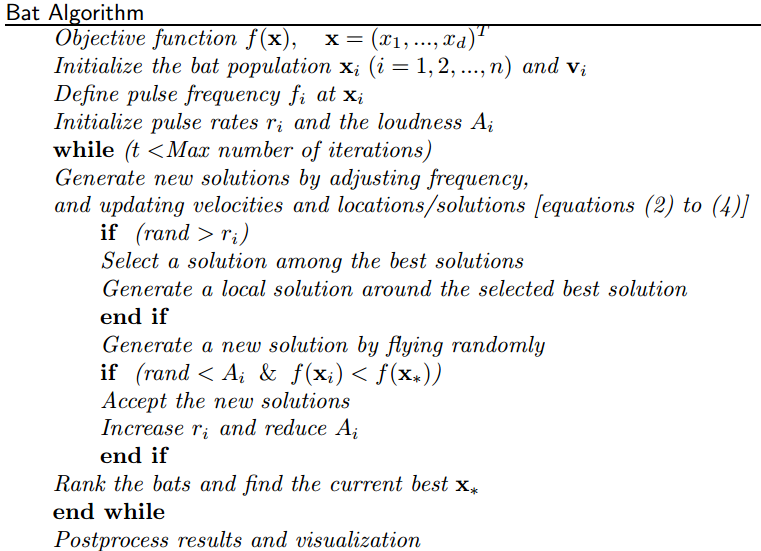
\includegraphics[width=1.0\textwidth]{algoritmo-bat.png}
          \caption{Algoritmo de ecolocalização de morcegos \cite{bat}}
      \end{figure}
  \end{frame}

  \begin{frame}{Estridência e emissão de pulsos}
      À medida que o algoritmo avança, é necessário atualizar a estridência $A_i$ e a taxa de emissão de pulsos $r_i$. Desta forma temos:
      \begin{equation}
          A^{t+1}_i = \alpha A^{t}_i, r^{t+1}_i = r^{0}_i[1 - e^{-\gamma t}]
      \end{equation}
      Onde $\alpha e \gamma$ são constantes em que $\alpha$ é similar ao fator de resfriamento do recozimento simulado;
  \end{frame}

  \begin{frame}{Experimentos e Resultados}
      Rosenbrock foi a função de benchmark utilizada:
      \begin{equation}
          f(x) = \sum \limits^{d-1}_{i=1} (1-x^{2}_i)^2 + 100(x_{i+1} - x^{2}_i)^2, -2048 \leq x \leq 2048
      \end{equation}
      E também a função eggcrate:
      \begin{equation}
          g(x,y) = x^2 + y^2 + 25(sin^2x + sin^2y), (x, y) \in [-2\pi, 2\pi] x [-2\pi, 2\pi]
      \end{equation}
      As funções tem mínimo global $f_{min} = 0$ em $(1,1)$ e $g(x,y)$ em $(0,0)$
  \end{frame}

  \begin{frame}{Eggcrate depois de 10 iterações}
      \begin{figure}
          \centering
          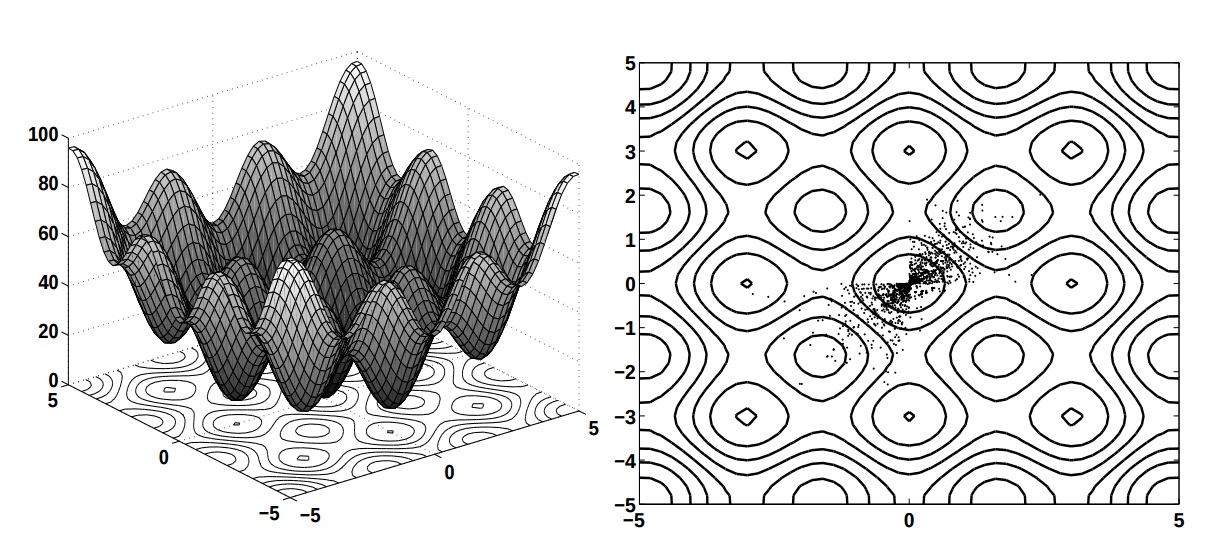
\includegraphics[width=1.0\textwidth]{eggcrate.png}
          \caption{Eggcrate depois de 10 iterações \cite{bat}}
      \end{figure}
  \end{frame}

  \begin{frame}{Resultados}
      \begin{figure}
          \centering
          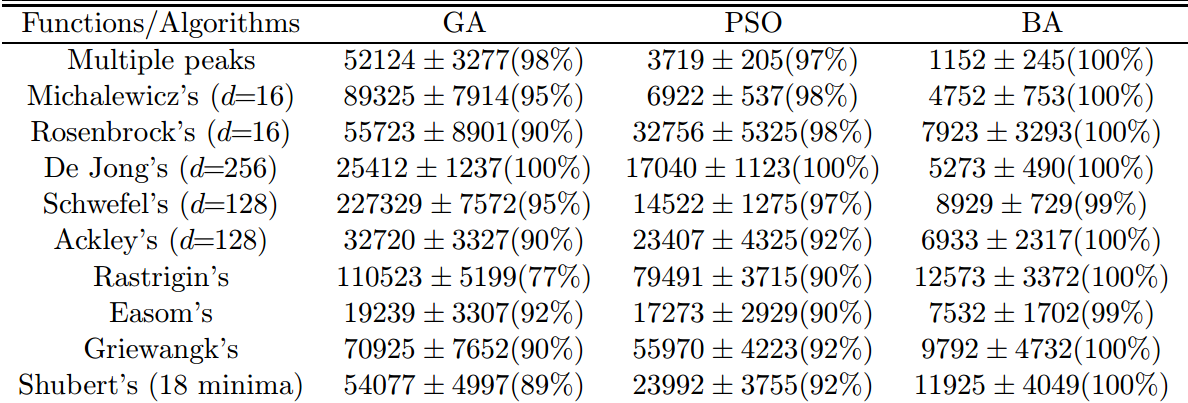
\includegraphics[width=1.0\textwidth]{comparacao.png}
          \caption{Comparação dos resultados \cite{bat}}
      \end{figure}
  \end{frame}

  \begin{frame}{Proposta de melhoria}
      É uma tarefa difícil tentar melhorar resultados bons. A abordagem sugerida é a de introduzir uma pertubação aleatória na voz do morcego com o intuito de desorienta-lo e o espaço de busca local ser melhor explorado. Tal técnica é inspirada na mutação dos algoritmos genéticos. Logo, a estridência pode ser remodelada da seguinte forma:
      \begin{equation}
          A^{t+1}_i = \alpha A^{t}_i+N(-1,1)
      \end{equation}
      Em que N é um gerador de números aleatórios baseado em uma distribuição normal.
  \end{frame}


  \section{Perguntas}
  \section{Muito obrigado!}

  \begin{frame}
      \bibliographystyle{apacite}
      \bibliography{apresentacao}
  \end{frame}
\end{document}
